\subsection{Sequence diagram}
To get an overview of the entire architecture a sequence diagram has been made. The diagram shows the communication between the bricks and their respective sensors and motors. The entire sequence diagram can be seen in \appref{app:sequence-diagram}.

\subsubsection{Initialisation phase}
The first part of the sequence diagram shows the initialising phase along with the constant loops the continues throughout the entire running period. 

\begin{figure}[H]
     \center{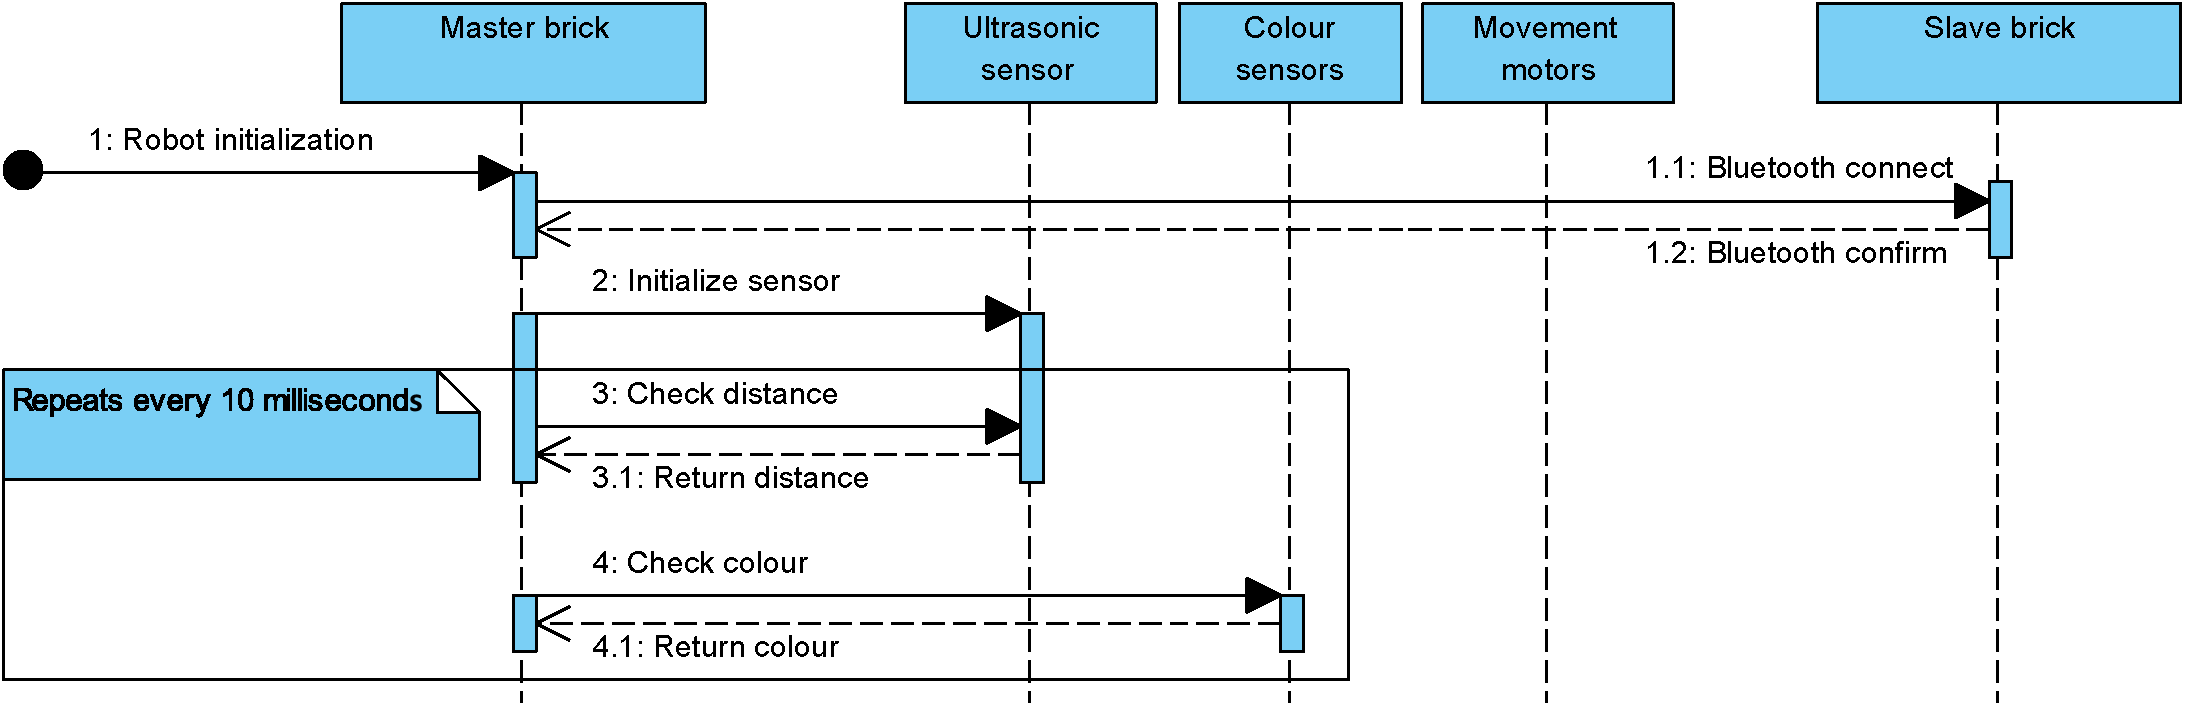
\includegraphics[width=\textwidth]
     {graphics/SequenceDiagramInitialization.png}}
     \caption{\label{fig:sequence-diagram-initialisation-appendix} Initialisation snip of the full sequence diagram.}
\end{figure}

\figref{fig:sequence-diagram-initialisation-appendix} shows the initialisation process. At first the master unit connects to the slave unit and confirms that the connection exist. Then the master unit initialises the sensors and enter a loop, which repeat itself every 10 milliseconds. 

\subsubsection{Object spotting phase}
The second part of the sequence diagram shows the object spotting phase along with a loop which continues as long as an object is spotted and not within reaching distance.

\begin{figure}[H]
     \center{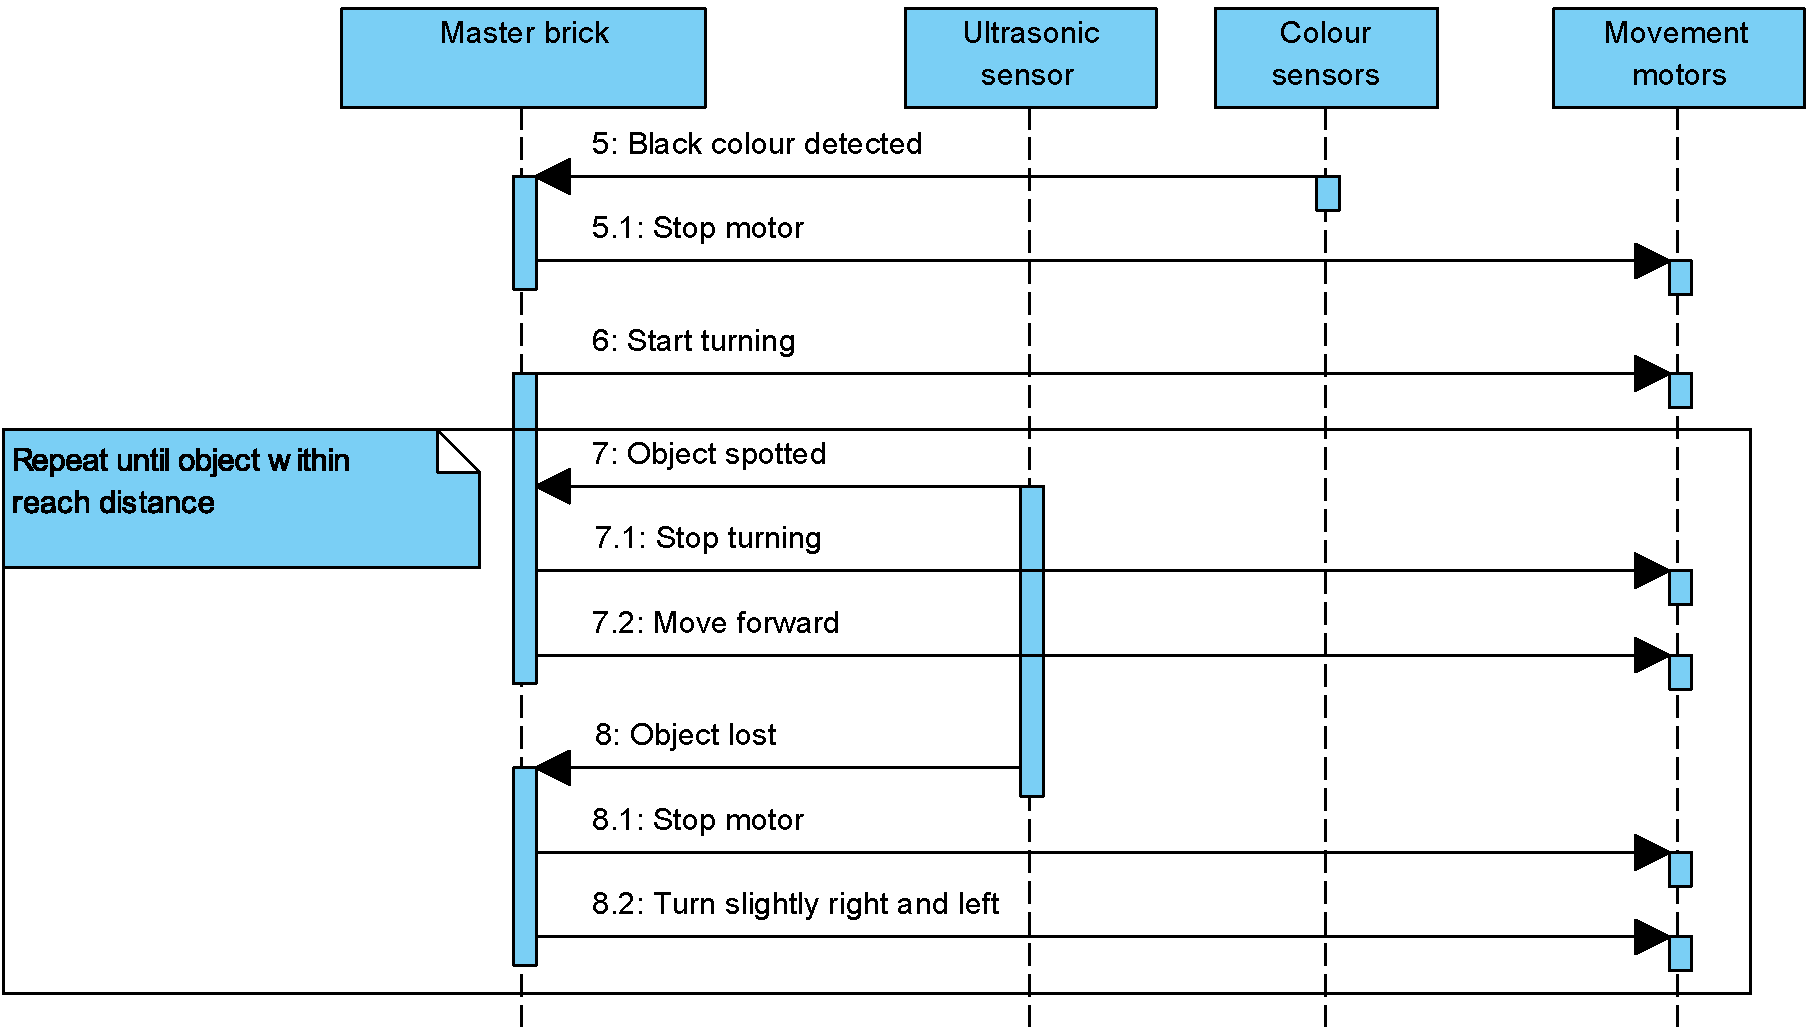
\includegraphics[width=\textwidth]
     {graphics/SequenceDiagramObject.png}}
     \caption{\label{fig:sequence-diagram-object-appendix} Object snip of the full sequence diagram.}
\end{figure}

\figref{fig:sequence-diagram-object-appendix} shows the spotting process. If a black colour is detected, the motors are stopped, then it drives backwards a few centimeters and then continues turning. If on the other hand an object is spotted it stops turning and start to move forward towards the object, while repeatably scanning for the object and checking for the boundary. If the object is out sight, it stops and turns slightly to each side until the object is in sight again. During this phrase, the loop checking distance and colour sensor input is running alongside it. \fxnote{Fix sequence diagram, med at vi bakker, når vi møder den sorte farve}

\subsubsection{Slave}
The \figref{fig:sequence-diagram-slave-appendix} shows how the slave unit works. The slave unit's overall task is to collect an object from the floor. The slave unit starts when it receives a command from the master unit. When the command is received the claw motor closes and the arm motor turns towards the storage unit. After this process the claw motor and arm motor return to the start position.

\begin{figure}[H]
     \center{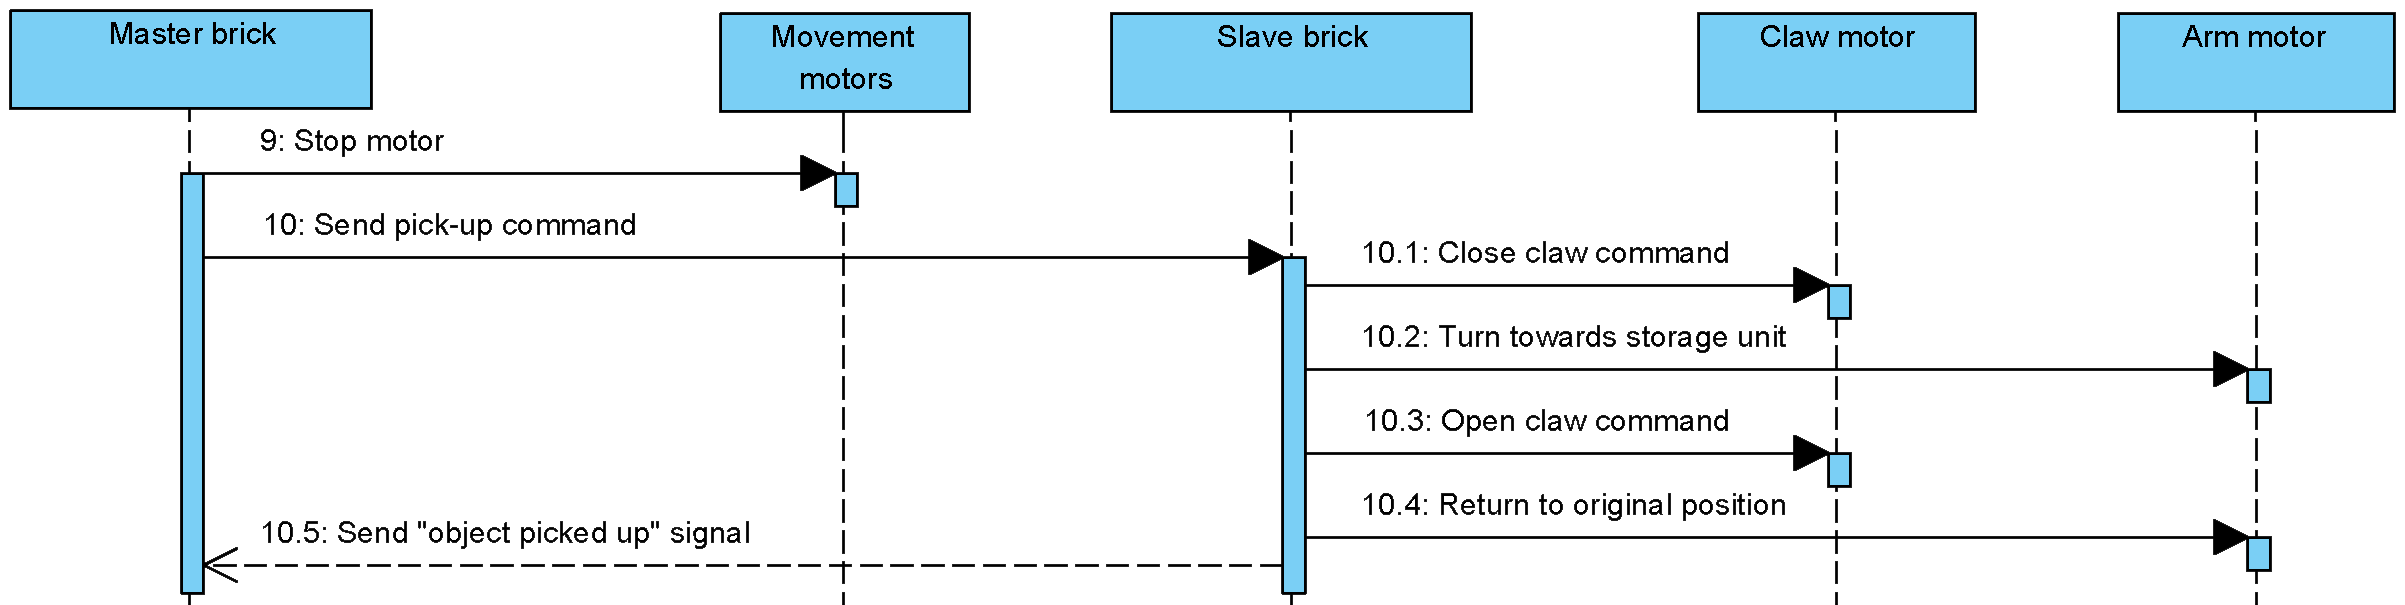
\includegraphics[width=\textwidth]
     {graphics/SequenceDiagramSlave.png}}
     \caption{\label{fig:sequence-diagram-slave-appendix} Slave brick snip of the full sequence diagram.}
\end{figure}
